\documentclass[12pt, a4paper,oneside]{report}



\usepackage{titlesec}
\usepackage[utf8]{inputenc}
\usepackage[american]{babel}
\usepackage[T1]{fontenc}
\usepackage{textcomp}
\usepackage{framed}
\usepackage{pbox}
\usepackage{caption}
\usepackage[nottoc,numbib]{tocbibind}
\usepackage[pdftex]{graphicx}
\usepackage[toc]{glossaries}
\usepackage{amssymb, amsmath}
\usepackage[colorlinks,
pdfstartview = FitH,
linkcolor = black,
plainpages = false,
hypertexnames = false,
citecolor = black]{hyperref}
\usepackage{setspace}
\onehalfspacing
\usepackage[left=3.5cm,right=3.5cm,top=2cm,bottom=2cm]{geometry}
\graphicspath{{./pics/}}
\usepackage[printonlyused]{acronym}
\usepackage{todonotes}
\usepackage{subcaption}
\usepackage{float}
\usepackage{pifont}
\newcommand{\cmark}{\ding{51}}%
\newcommand{\xmark}{\ding{55}}%
\usepackage{multirow}
\usepackage{pdflscape}
\usepackage{eurosym}
\usepackage{url}
\usepackage{etoolbox}


\usepackage{tocbibind}



\parindent 0pt

\begin{document}

\begin{titlepage}
	University Passau\newline
	Faculty of Computer Science and Mathematics
	\vspace{2.5cm}
    \begin{center}
    \LARGE\textbf{\textsc{Bachelor Thesis}}\\
    \vspace{1cm}
    \huge \textbf{\textsf{Privacy Model Substitution}} \\
    \vspace{1cm}
    \normalsize

    \vspace{2.5cm}
    \end{center}

 \normalsize{
 	Thesis Prepared for the Degree of\newline
 	Bachelor of Science (B.Sc.)\newline
 	\ \\
 	at the Chair of Distributed Information Systems \newline
 	of the Faculty of Computer Science and Mathematics\newline
 	of the University Passau\newline

    \begin{tabular}{ll}
    	Name: & Fabian Pfeil \\
    	Matriculation Number: & 77560 \\
    	Subject Area: & Computer Science\\
    	Course of studies: & Bachelor Internet Computing\\
    	Schwerpunkt: & TODO \\
    	Studienjahrgang: & TODO \\
	Erstprüfer: & Prof. Dr. NN \\
	Zweitprüfer: & Prof. Dr. NN2 \\ 
    \end{tabular}\\
    }


\end{titlepage}


\setcounter{tocdepth}{10}
\tableofcontents


% \begin{acronym}

% \acro{XML} {Extensible Markup Language}s

% \end{acronym}


\listoffigures
\listoftables

\titleformat{\chapter}{\LARGE\bfseries}{\thechapter}{1em}{}




\chapter*{Abstract}

Zitiertest\cite{Gerl2018}.\\
K-anonymity\cite{SWEENEY2002}.\\
L-diversity\cite{Machanavajjhala2006}.\\
T-closeness\cite{Li2007}.\\
d-presence\cite{Nergiz2007}\\
delta-disclosure\cite{Brickell2008}\\
basic-beta-likeness\cite{Cao2012}\\
k-map1\cite{Emam2008}\\
population uniqueness\cite{Dankar2012}\\
profitability 1\cite{Wan}\\
profitability 2\cite{Prasser2017}\\
arx\cite{arx}\\
diff\cite{Dwork2006}\\
diff2\cite{Bild2018}\\
diff3\cite{Li2012}\\

\newpage
\chapter{Introduction}

\section{Motivation}

\begin{figure}[!ht]
	\centering
% remove these comments to insert picture at img/file.png
% \includegraphics[width=1.0\textwidth]{img/file.png}
	\caption{Describe this picture.}
	\label{fig:1}
\end{figure}

\section{Layered Privacy Language}

\chapter{Privacy Model Classification}\label{class}
In this section, we will take a look at the Privacy Models implemented by Arx. Therefore, these Privacy Models will be explained in terms of requirements for the data sets to which they can be applied, the attacks they mitigate, their use cases, advantages and disadvantages.

\section{Definitions}

\section{K-Anonymity} 
The first Privacy Model, we will take a look at is K-Anonymity. This Privacy Model was released in 2002 by Latanya Sweeney with the goal to prevent re-identification of data subjects of certain data sets\cite{SWEENEY2002}. K-Anonymity is defined as follows:\\
\par
\begingroup
\leftskip4em
\rightskip\leftskip
"Let RT(A\textsubscript{1},...,A\textsubscript{n}) be a table and QI\textsubscript{RT} be the quasi-identifier associated with it. RT is said to satisfy k-anonymity if and only if each sequence of values in
RT[QI\textsubscript{RT}] appears with at least k occurrences in RT[QI\textsubscript{RT}]."\cite{SWEENEY2002}\\
\par
\endgroup
To clarify what this means, figure \ref{fig:2} shows the example used in Sweeney's work\cite{SWEENEY2002}.  
\begin{figure}[h]
	\centering
	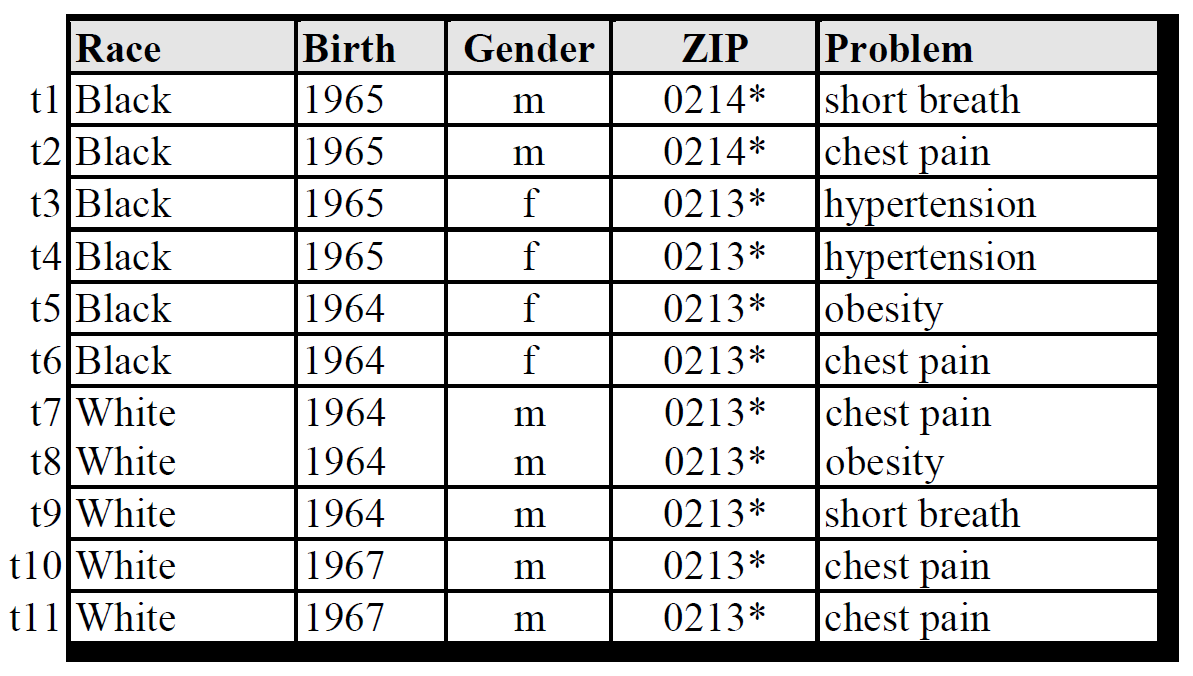
\includegraphics[width=0.8\textwidth]{k-anonymity-example}
	\caption{Example of a 2-anonymous table \cite{SWEENEY2002}}
	\label{fig:2}
\end{figure}
The figure shown here, is an example for a table that satisfies the k-anonymity criterion. The quasi-identifier for this particular case is QI\textsubscript{T}= \{Race, Birth, Gender, ZIP\} and k = 2. This means that every tuple of quasi-identifying attributes appears at least in two records in T.\\
As k-Anonymity is defined, we will now take a look at the attacks, which can be mitigated with the property of k-anonymity applied. As this issue was already addressed by Fung et al., their classification will be used here. In the work of Fung et al. it is stated that k-anonymity, applied to a data set, will prevent only Record Linkage attacks. Consequently, other attacks like Attribute Linkage, Table Linkage or a Probabilistic Attack can not be mitigated by k-Anonymity\cite{Fung2010}.

\subsection{K-Map}
The Privacy Model of K-Map is directly related to k-Anonymity. El Emam et al. show that extending k-Anonymity to k-Map can however reduce the loss of information due to over-anonymization of the dataset\cite{Emam2008}. Damien Desfontaines describes k-Map like this: "Your data satisfies k-map if every combination of values for the quasi-identifiers appears at least k times in the reidentification dataset."\cite{desfontaines}\\
The similarity to k-Anonymity is obvious, as the main criterion in both Privacy Models is the same, the only difference is the data set on which they are based. In the case of k-Map it is not the data set of the data custodian, it is the reidentification dataset\cite{desfontaines}. Consequently, K-Map mitigates the same attacks (Record Linkage Attacks) as k-Anonymity. Other attacks can not be prevented by this Privacy Model.\\
However, the work of El Emam et al. states, that even though k-Map reduces information loss in comparison to k-Anonymity, the model of k-Map is not used in practices because one can assume that a data custodian does not have access to a reidentification dataset, while an attacker does\cite{Emam2008}.  

\section{l-Diversity}

The next Privacy Model we will take a look at is l-Diversity. L-Diversity was proposed by Machanavajjhala et al. to overcome the weaknesses of k-Anonymity, namely the attribute linkage attacks\cite{Machanavajjhala2006}. To understand why l-Diversity mitigates attribute linkage, we will take a short look at the definition. In the work of Machanavajjhala et al. the principle of l-Diverity is defined as follows:
\pagebreak
\par
\begingroup
\leftskip4em
\rightskip\leftskip
"A $q^*$-block is l-diverse if it contains at least l well-represented values for the sensitive attribute S. A table is l-diverse if every $q^*$-block is l-diverse." \cite{Machanavajjhala2006}\\
\par
\endgroup
This means that every group of quasi-identifiers has to at least contain l different values for the sensitive attribute S. It is because of this property that l-diversity can prevent attribute linkage attacks. However, table linkage attacks can not be mitigated through l-diversity\cite{Fung2010}. Machanavajjhala et al. use the table shown in figure \ref{fig:3} as an example for l-diversity. In this example, one can see that every group of quasi-identifiers contains at least three different values for the sensitive attribute.
\begin{figure}[h]
	\centering
	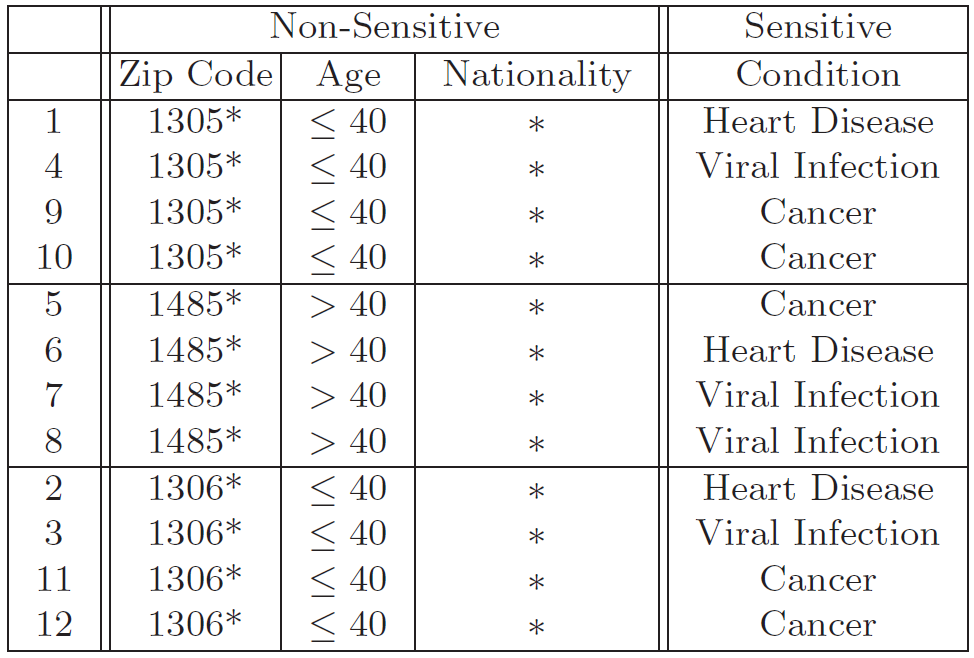
\includegraphics[width=0.8\textwidth]{l-diversity-example}
	\caption{Example of a 3-diverse table \cite{Machanavajjhala2006}}
	\label{fig:3}
\end{figure}\\
There are three instantiations of l-diversity implemented in Arx. Consequently, we will only take a look at these. 

\subsection{Distinct-l-Diversity}

Distinct-l-Diversity is arguably the simplest of the three instantiations of l-diversity. It is also known as p-sensitive k-anonymity. Distinct-l-diversity uses the plain definition of l-diversity mentioned above. Therefore, no advanced calculation of the l-factor has to take place. One can simply take the number of different values of the sensitive attribute as the factor l\cite{Fung2010}.\\
Lets get back to our example in figure \ref{fig:3}. With distinct-l-diversity the table shown here is, as simple as it sounds, 3-diverse because every group of quasi-identifiers has three different values. Consequently, this table is diverse.\\ 
With this form of l-diversity, probabilistic inference attacks cannot be mitigated, because of the fact that some values of sensitive attributes are more frequent than others. Therefore, two stronger instantiations of l-diversity have been created\cite{Fung2010}. 

\subsection{Entropy-l-Diversity}

The next instantiation of l-Diversity is Entropy-l-Diversity. It is defined as follows:
\par
\begingroup
\leftskip4em
\rightskip\leftskip
"A table is Entropy l-Diverse if, for every $q^*$-block,\\
\[ - \sum_{s \in S}^{}p(q^*, s')log(p(q^*, s')) \geq log(l)\]\\
where \[ p(q^*, s) = \frac{n(q^*, s)}{\sum_{s' \in S}^{}n(q^*, s')} \] is the fraction of tuples in the $q^*$-block with sensitive
attribute value equal to s."\cite{Machanavajjhala2006}\\
\par
\endgroup
 With this calculation of the l-factor for our example in figure \ref{fig:3}, our table is actually 2.8-diverse. Consequently, every group of quasi-identifiers has at least 2.8 different values for the sensitive attribute. And as there can not be 2.8 different values there are in our case three existing values.

\subsection{Recursive (c, l)-Diversity} \label{ssrec}

The third and final instantiation of l-Diversity we will take a look at is the recursive (c, l)-Diversity. This privacy model makes sure, that the most frequent values of sensitive attributes do not appear to often in the table. Furthermore it makes the uncommon values appear not too rarely\cite{Fung2010}. Machanavajjhala et al. define recursive (c, l)-Diversity like this: \\
\par
\begingroup
\leftskip4em
\rightskip\leftskip
"In a given $q^*$-block, let $r_i$ denote
the number of times the $i^{th}$ most-frequent sensitive value appears in that $q^*$-block. Given a constant c, the $q^*$-block satisfies recursive (c, l)-diversity if r1 > c($r_l$ + $r_{l+1}$ + ... + $r_m$). A table $T^*$ satisfies recursive (c, l)-diversity, if every $q^*$-block satisfies recursive l-diversity. We say that 1-diversity is always satisfied."\cite{Machanavajjhala2006}\\
\par
\endgroup

Both of these definitions for l-diversity, entropy and recursive, may be too restrictive. For entropy-l-diversity this can bee seen in the fact that, if entropy l-diversity should be applied, the entropy of whole table has to be log(l) or higher. This may be very difficult to achieve when, for example, a value for a sensitive attribute is too common.\\
The same is the case for recursive (c, l)-Diversity. When for example a sensitive attribute value is present 90\% of the time and the factor c is chosen $<$ 9, it is impossible to achieve recursive (c, l)-Diversity\cite{Machanavajjhala2006}.\\
This is not the only Problem with l-Diversity. Sensitive information can be leaked, despite the fact that l-diversity is applied, because l-diversity only  guarantees the diversity of sensitive attribute values, but does not take the semantical relations of these values into account. Consequently, l-Diversity is insufficient to prevent attribute linkage in some cases where the distribution of a sensitive attribute is skewed\cite{Li2007}.    

\section{t-Closeness}

The next privacy model is t-Closeness. It was proposed by Li et al. to prevent attribute linkage through skewness attacks, mentioned earlier in section \ref{ssrec} \cite{Li2007}. In the work of Li et al. the property of t-Closeness is defined as follows: \\
\par
\begingroup
\leftskip4em
\rightskip\leftskip
"An equivalence class is said to have t-closeness if the distance between the
distribution of a sensitive attribute in this class and the distribution of the attribute in the whole table is no more than a threshold t. A table is said to have t-closeness if all equivalence classes have t-closeness."\cite{Li2007}\\
\par
\endgroup

The factor t can be used to manage a trade off between privacy and utility. To measure the distance between those distributions and to compute the t-factor, Li et al. use the Earth Mover's Distance (EMD). In the work of Li et al, certain formulas were derived to calculate the EMD for the cases we will consider in the following subsections of t-closeness\cite{Li2007}.

\subsection{Ordered Distance t-Closeness}

This type of t-closeness is used for numerical attributes, as these can be ordered. The distance between the distributions (in this case P and Q, with $r_i = p_i - q_i, (i = 1,2,...m)$) is calculated as follows \cite{Li2007}:

\[ D[P,Q] = \frac{1}{m-1}(|r_1| + |r_1 + r_2| +...+ |r_1 + r_2 +...r_{m-1}|) =  \frac{1}{m-1}\sum_{i=1}^{i=m}\Biggl|\sum_{j=1}^{j=i}r_j\Biggl| \]


\subsection{Equal Distance t-Closeness}

Some types of attributes can not be orered like numerical values. Therefore, the next two computations of the EMD are used for categorical attributes, as they can not be ordered.\\
With the equal distance approach, all distances between any two values of categorical attributes are considered to be 1. Consequently, the following formula to compute the distance is the result\cite{Li2007}:

\[ D[P,Q] = \frac{1}{2}\sum_{i=1}^{m}|p_i-q_i| = \sum_{p_i \ge q_i}^{}(p_i-q_i) = - \sum_{p_i < q_i}^{}(p_i-q_i) \]

\subsection{Hierarchical Distance t-Closeness}

Another way to compute the distance between distributions of categorical values is the hierarchical distance approach. This technique bases the distances of values on the minimum level to which these two values can be generalized to, based on a domain hierarchy\cite{Li2007}.\\ Therefore, the so called extra of a leaf of this hierarchy is defined as: 
\[ extra(N) = \begin{cases} p_i - q_i & \text{if N is a leaf} \\ \sum_{C\in Child(N)}^{}extra(C) & \text{otherwise} \end{cases} \]
where Child(N) is the portion of leaf nodes below N. Furthermore, two additional functions for internal Nodes are defined:
\[ pos\_extra(N) = \sum_{C\in Child(N)\wedge extra(C)>0}^{}|extra(C)|\]
\[ neg\_extra(N) = \sum_{C\in Child(N)\wedge extra(C)<0}^{}|extra(C)|\]
This leads to the cost-function, which describes the cost of moving between some leaf's (N) children branches.
\[ cost(N) = \frac{height(N)}{H}min(pos\_extra(N),neg\_extra(N)) \]
Finally, the EMD can be seen as follows:
\[  D[P,Q] = \sum_{N}^{}cost(N) \]
Now that we have defined the special cases for t-closeness, we will take a look at a short example used by Li et al. in their work\cite{Li2007}.
\begin{figure}[h]
	\centering
	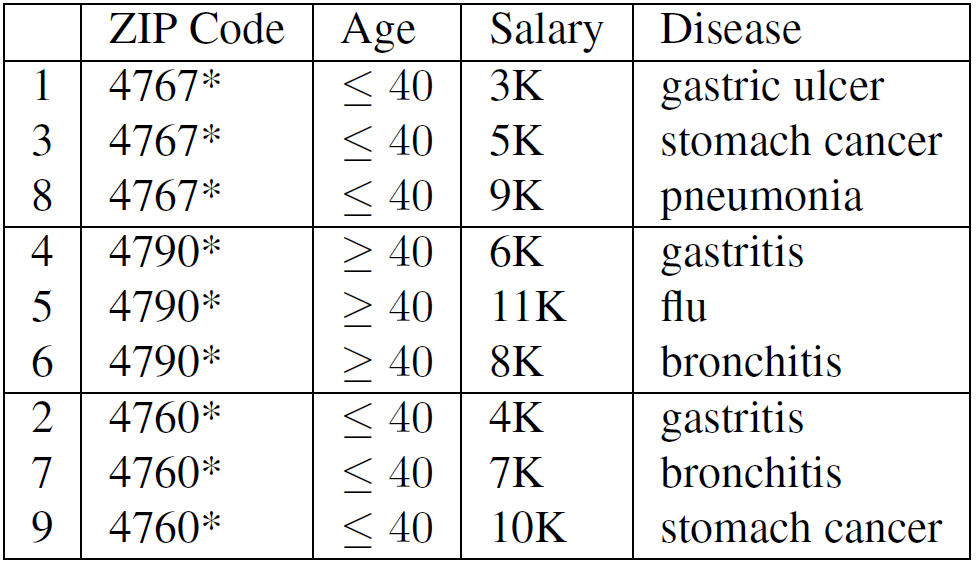
\includegraphics[width=0.8\textwidth]{t-closeness-example}
	\caption{Table that has 0.167-closeness w.r.t.
	Salary and 0.278-closeness w.r.t. Disease \cite{Li2007}}
	\label{fig:4}
\end{figure}\\
Figure \ref{fig:4}, shows a Table which has 0.167-closeness in relation to the sensitive attribute Salary, which can be calculated using the ordered distance formula for numerical values, and 0.278-closeness in relation to the attribute Disease. This can be easily computed using the given domain hierarchy shown in figure \ref{fig:5}.   
\begin{figure}[h]
	\centering
	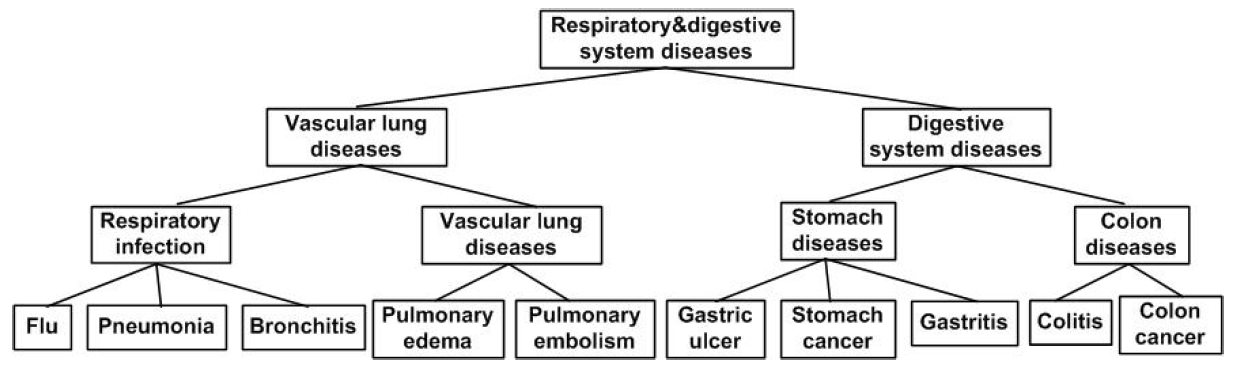
\includegraphics[width=1.0\textwidth]{hierarchy-t-close}
	\caption{Hierarchy for categorical attributes Disease \cite{Li2007}}
	\label{fig:5}
\end{figure}

\section{delta-Disclosure privacy}

The next privacy model is delta-disclosure privacy. It also can be used to protect data sets from attribute linkage attacks, due to the fact that it is related to the t-closeness model. It also enforces restrictions on the distances between the sensitive attribute distributions. In contrast to the model proposed by Li et al., delta-disclosure privacy uses a multiplicative approach, which makes it stricter than t-closeness\cite{Brickell2008}. \\
Delta-disclosure privacy was proposed by Brickell et al. and is defined as follows: \\
\par
\begingroup
\leftskip4em
\rightskip\leftskip
"We say that an equivalence class $\langle t\rangle$ is $\delta$-disclosure-private with regard to the sensitive attribute S if, for all s $\in$ S
\[ A_{quot}(\langle t\rangle) = \Biggl| log\frac{p(\langle t\rangle,s)}{p(T,s)} \Biggl| < \delta \]
A table T is $\delta$-disclosure-private if for every t $\in$ $E_Q$, $\langle t\rangle$ is $\delta$-disclosure private."\cite{Brickell2008}\\
\par
\endgroup

In easier words, one can say that a table T is delta-disclosure private if the distributions of sensitive attributes in the equivalence classes and in the overall table are approximately the same\cite{Brickell2008}.

\section{beta-Likeness}

The privacy model beta-Likeness tries to overcome the limitations of the previous two models, as the EMD in t-closeness does not provide a clear privacy guarantee and the delta-disclosure privacy requires that every value of a sensitive attribute of the overall table occurs in every equivalence class. This makes delta-disclosure privacy unnecessarily strict.\\
To avoid these disadvantages, Cao et al. propose a privacy model called beta-Likeness. This model assumes that the distribution of the sensitive attributes in a table are known to the public and bases it's privacy constraint on information gain, which is denoted as a difference function between the distribution of a sensitive attribute in the overall table and in an equivalence class\cite{Cao2012}.\\
In the work of Cao et al., two instantiations of beta-Likeness are introduced.   

\subsection{basic beta-Likeness}

The base approach for beta-likeness is defined as follows:\\
\par
\begingroup
\leftskip4em
\rightskip\leftskip
"Given table DB with sensitive attribute SA, let V = \{$v_1$, ... , $v_m$\} be the SA domain, and P = ($p_1$, ... , $p_m$) the overall SA distribution in DB. An EC G with SA distribution Q = ($q_1$, . . . , $q_m$) is said to satisfy basic $\beta$-likeness, if and only if $max\{D(p_i, q_i)|p_i \in P, p_i < q_i\} \le \beta,$ where  $\beta > 0$ is a threshold."\cite{Cao2012}\\
\par
\endgroup

This means, that every distance between the distributions of sensitive attributes in the overall table and in the equivalence class has to be lower or equal to a certain threshold $\beta$.\\
Furthermore, Cao et al. state that every equivalence class of an anonymized table satisfies beta-likeness, the whole table obeys beta-likeness.\\
The distance function for this privacy model is defined as $D(p_i,q_i) = \frac{q_i - p_i}{p_i}$ as Cao et al. opt for a relative difference instead of a absolute difference, because it does not suite their purposes. This relative distance function pays attention to less frequent values of sensitive attributes. Consequently, sensitive attribute values with a large frequency were not put into consideration. To mitigate the privacy threat caused by this, Cao et al. provide a stronger definition of beta-Likeness\cite{Cao2012}.     

\subsection{Enhanced beta-Likeness}

This instantiation of beta-Likeness is stronger than basic beta-Likeness, as the name suggests. Enhanced beta-Likeness is defined as follows:\\

\par
\begingroup
\leftskip4em
\rightskip\leftskip
"For table DB with sensitive attribute SA, let V = \{$v_1$, ... , $v_m$\} be the SA domain, and P = ($p_1$, ... , $p_m$) the overall SA distribution in DB. An EC G with SA distribution Q = ($q_1$, ... , $q_m$) is said to satisfy enhanced $\beta$-likeness, if and only if $\forall q_i, D(p_i, q_i) = \frac{q_i-p_i}{p_i} \le min\{\beta,-\text{ln}p_i\}$, where $\beta$ > 0 is a threshold and ln $p_i$ is the natural logarithm of $p_i$."\cite{Cao2012}\\
\par
\endgroup

The properties that come with this definition protect the privacy for al sensitive attribute values. Values with rare occurrence receive sufficient attention, while values that occur more often can not approach frequency values of 1. As it is more robust than basic beta-likeness in terms of privacy, it should be used instead of it's predecessor\cite{Cao2012}.\\
Due to these traits and the fact that it is related to t-closeness and delta-disclosure privacy, the privacy model of beta-likeness can protect data sets against attribute linkage attacks.

\section{delta-Presence}

The next privacy model that we take into consideration is delta-Presence. This model was proposed by Nergiz et al. to prevent attacks from identifying that a certain suspect is part of a dataset (Table Linkage), as this can pose a serious privacy threat in certain cases\cite{Nergiz2007}.\newpage
The privacy model of delta-presence is defined as follows:\\
\par
\begingroup
\leftskip4em
\rightskip\leftskip
"Given an external public table P, and a private table T , we say that $\delta$-presence holds for a generalization T* of T, with $\delta$ = ($\delta_{min},\delta_{max}$) if
\[ \delta_{min} \le P(t \in T|T*) \le \delta_{max} \quad \forall t \in P"\cite{Nergiz2007}\]
\par
\endgroup

In a dataset which applies this privacy criterion, every tuple t is called $\delta$-present within the range of $\delta = (\delta_{min}, \delta_{max})$. To clarify what this means, we will take a short look at the example used in the work of Nergiz et al.\\
In Figure \ref{fig:6} the tables $P*_3$ and $T*_3$ are given. To get the probabilities $\delta_{min}, \delta_{max}$, the following calculations are done. $P(a \in T | T*_3) = \frac{|{b,c,f}|}{|{a,b,c,d,e,f}|} = \frac{1}{2}$. The same is done for tuples b,c,d,e and f. The probability for the tuples g,h and i is calculated with $\frac{|{h,i}|}{|{g,h,i}|} = \frac{2}{3}$. Consequently, the probability that a tuple from Table $P*_3$ is also in $T*_3$ lies between $\frac{1}{2}$ and $\frac{2}{3}$.\\  
Like in most privacy models the $\delta$-factor can be used as a trade-off between privacy and utility. Therefore this factor has to be chosen carefully. 
\begin{figure}[h]
	\centering
	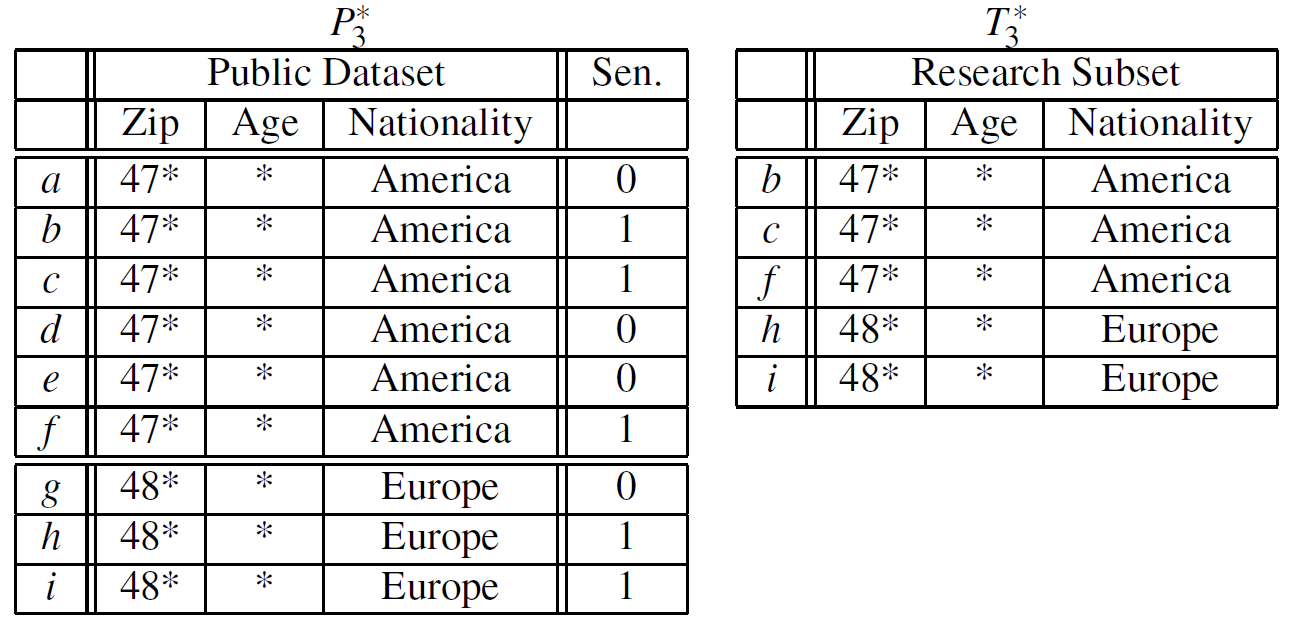
\includegraphics[width=0.8\textwidth]{d-presence-example}
	\caption{Table $T*_3$ that is ($\frac{1}{2}, \frac{2}{3})$-present  \cite{Nergiz2007}}
	\label{fig:6}
\end{figure}


\subsection{Inclusion}

Only mentioned in Github arx, allows to define a subset. 

\section{Profitability}

4 models, prosecutor and journalist with each normal an no attack, SH and 0 risk scenario corresponding to k-anonymity and k-map

\section{Differential privacy}

first proposed by dwark. presence or absence of record does not effect the output, privacy not an attribute of a dataset, but of the data processing method, Attacks mitigated taken from arx, based on e-differential
privacy, (e, d)-differential privacy allows for higher data quality

\section{Average risk}

\section{Population uniqueness}

\section{Sample uniqueness}

\section{Classification Table}

The results from chapter \ref{class} are shown in the following classification table. The attacks mitigated by each privacy model are displayed here in table \ref{table:1}.
\newpage
\begin{table}[]
	\centering
	\resizebox{\textwidth}{!}{%
		\begin{tabular}{|l|c|c|c|c|}
			\hline
			\multicolumn{1}{|c|}{\multirow{2}{*}{Privacy Models}} & \multicolumn{4}{c|}{Attacks Model}                                                                                                                                                                                                                                                                                                      \\ \cline{2-5} 
			\multicolumn{1}{|c|}{}                                & \multicolumn{1}{r|}{\begin{tabular}[c]{@{}r@{}}Record\\ Linkage\end{tabular}} & \multicolumn{1}{l|}{\begin{tabular}[c]{@{}l@{}}Attribute\\  Linkage\end{tabular}} & \multicolumn{1}{l|}{\begin{tabular}[c]{@{}l@{}}Table\\ Linkage\end{tabular}} & \multicolumn{1}{l|}{\begin{tabular}[c]{@{}l@{}}Probabilistic\\ Attack\end{tabular}} \\ \hline
			k-Anonymity                                           & X                                                                              &                                                                                   &                                                                              &                                                                                     \\ \hline
			k-Map                                                 & X                                                                              &                                                                                   &                                                                              &                                                                                     \\ \hline
			Distinct-l-Diversity                                  & X                                                                              & X                                                                                 &                                                                              &                                                                                     \\ \hline
			Entropy-l-Diversity                                   & X                                                                              & X                                                                                 &                                                                              &                                                                                     \\ \hline
			Recursive (c, l)-Diversity                            & X                                                                              & X                                                                                 &                                                                              &                                                                                     \\ \hline
			Ordered Distance t-Closeness                          &                                                                                & X                                                                                 &                                                                              & X                                                                                   \\ \hline
			Equal Distance t-Closeness                            &                                                                                & X                                                                                 &                                                                              & X                                                                                   \\ \hline
			Hierarchical Distance t-Closeness                     &                                                                                & X                                                                                 &                                                                              & X                                                                                   \\ \hline
			delta-Disclosure Privacy                              &                                                                                & X                                                                                 &                                                                              & X                                                                                   \\ \hline
			Basic beta-Likeness                                   &                                                                                & X                                                                                 &                                                                              & X                                                                                   \\ \hline
			Enhanced beta-Likeness                                &                                                                                & X                                                                                 &                                                                              & X                                                                                   \\ \hline
			delta-Presence                                        &                                                                                &                                                                                   & X                                                                            &                                                                                     \\ \hline
			Inclusion                                             &                                                                                &                                                                                   &                                                                              &                                                                                     \\ \hline
			Profitability Prosecutor                              & X                                                                              &                                                                                   &                                                                              &                                                                                     \\ \hline
			Profitability Journalist                              & X                                                                              &                                                                                   &                                                                              &                                                                                     \\ \hline
			Profitability Prosecutor No Attack                    & X                                                                              &                                                                                   &                                                                              &                                                                                     \\ \hline
			Profitability Journalist No Attack                    & X                                                                              &                                                                                   &                                                                              &                                                                                     \\ \hline
			(e, d)-differential Privacy                           & X                                                                              & X                                                                                 & X                                                                            &                                                                                     \\ \hline
			Average Risk                                          & X                                                                              &                                                                                   &                                                                              &                                                                                     \\ \hline
			Population Uniqueness                                 & X                                                                              &                                                                                   &                                                                              &                                                                                     \\ \hline
			Sample Uniqueness                                     & X                                                                              &                                                                                   &                                                                              &                                                                                     \\ \hline
		\end{tabular}%
	}
\caption{Attacks mitigated by each privacy model}
\label{table:1}
\end{table}
 
\chapter{Evaluation of Privacy Models (Performance)}

\chapter{Privacy Model Substitution Table}

\chapter{Conclusion}







\bibliographystyle{plain}
\bibliography{biblio}

\newpage
\chapter*{Erklärung zur Bachelorarbeit}
Ich erkläre hiermit, dass ich die vorliegende Arbeit selbständig verfasst und keine anderen als die angegebenen Quellen und Hilfsmittel verwendet habe. \newline
\ \\
Die Arbeit wurde bisher keiner anderen Prüfungsbehörde vorgelegt und auch noch nicht veröffentlicht.\newline
\ \\
Passau, den <date>
\newline
\ \\
\ \\
<First Name, Last Name>
\end{document}
